\chapter{Opis projektnog zadatka}
		
		%\textbf{\textit{dio 1. revizije}}\\
		
		%\textit{Na osnovi projektnog zadatka detaljno opisati korisničke zahtjeve. Što jasnije opisati cilj projektnog zadatka, razraditi problematiku zadatka, dodati nove aspekte problema i potencijalnih rješenja. Očekuje se minimalno 3, a poželjno 4-5 stranica opisa.	Teme koje treba dodatno razraditi u ovom poglavlju su:}
		%\begin{packed_item}
			%\item \textit{potencijalna korist ovog projekta}
			%\item \textit{postojeća slična rješenja (istražiti i ukratko opisati razlike u odnosu na zadani zadatak). Dodajte slike koja predočavaju slična rješenja.} %dodaj slike %
			%\item \textit{skup korisnika koji bi mogao biti zainteresiran za ostvareno rješenje.}
			%\item \textit{mogućnost prilagodbe rješenja } 
			%\item \textit{opseg projektnog zadatka}
			%\item \textit{moguće nadogradnje projektnog zadatka}
		%\end{packed_item}
		
		%\textit{Za pomoć pogledati reference navedene u poglavlju „Popis literature“, a po potrebi konzultirati sadržaj na internetu koji nudi dobre smjernice u tom pogledu.}
		 \text Naš cilj je napraviti web aplikaciju "Autos" za iznajmljivanje vozila privatnim i poslovnim korisnicima. \par 
		 \text Cilj projekta je upoznavanje te praktična primjena postupaka oblikovanja programske podrške sa zadaćom ostvarenja zahtjeva ovog zadatka, shvaćanje važnosti i značenja projektne dokumentacije te stvaranje iste. Također, od važnosti je i što preciznija implementacija zahtjeva i poboljšanje vještina u svim područjima potrebnim za uspješno implementiranje zadatka. Uz standardno programiranje i rad dokumentacije, jedna od važnijih vještina koje ćemo dobiti je znanje o raspodjeli rada i iskustvo suradnje sa timom ljudi s ciljem ostvarenja zajedničkom projekta na osnovi zahtjeva. \par 
		 \text U poslovanju vezanim za iznajmljivanje automobila već postoji znatan broj tvrtki koje nude vrlo sličan model onom koji mi ostvarujemo. Priložen je jedan primjer. \par 
		 \text (izvor rentalcars.com)\par  
		 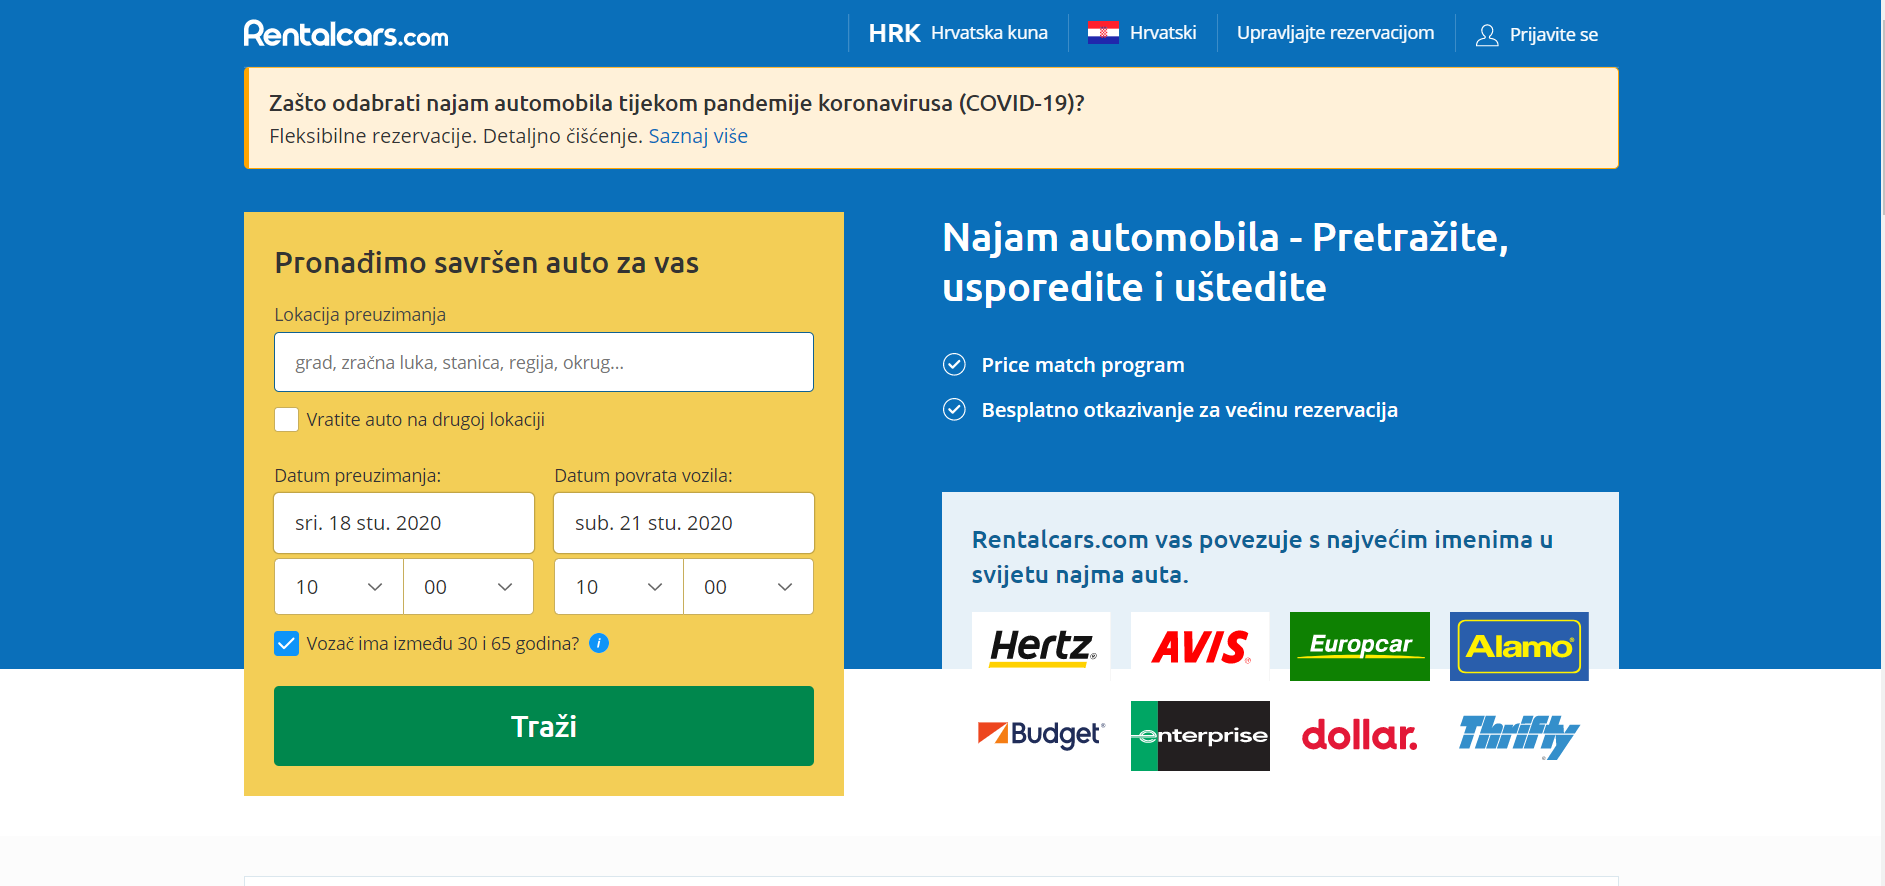
\includegraphics[scale=0.3]{slike/stranica1.png}
		 
		 \text Kao što vidimo u primjeru se nudi datum i vrijeme preuzimanja i vraćanja vozila te lokacija preuzimanja i vraćanja auta. Također se na stranicu moguće prijaviti i odabrati način plaćanja. \par 
		%\text (tu još jedna slika)
		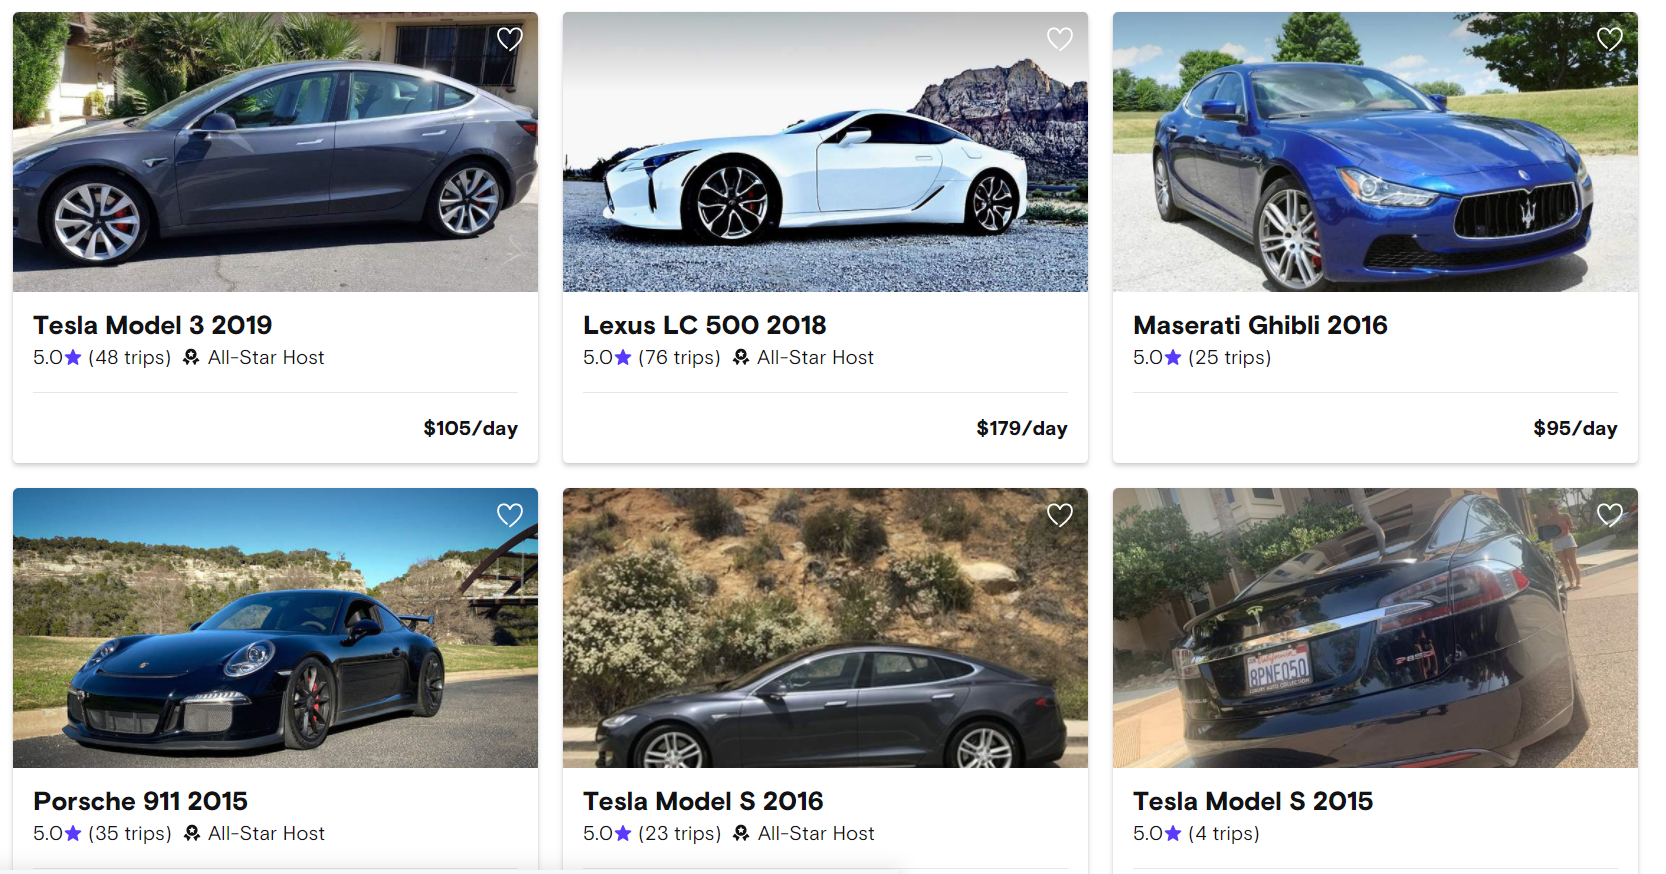
\includegraphics[scale=0.33]{slike/stranica2.png}
		
		 \text U ovom je primjeru vidljiv i izbor pojedinog automobila za iznajmljivanje. \par
		 \text (izvor turo.com) \par 
		 \text Godišnje oko 580 milijuna ljudi u svijetu koristi usluge iznajmljivanja  automobila, a od toga čak 70 je posto online. Ukupan broj korisnika ovih usluga kao i postotak online korištenja je u porastu te se nastavak tog porasta očekuje kroz sljedećih nekoliko godina. \par
		 \text Jedan od zahtjeva ovog zadatka je stvoriti mogućnost prijave te registracije korisnika za koju je potrebno ime, prezime,  naziv institucije ili poduzeća (za službene korisnike), adresa (ulica, kućni broj,
grad, država) i adresa elektroničke pošte. \par 
         \text Implementacija će sadržavati četiri različite vrste korisnika: administrator, vlasnik sustava,
korisnik (najmoprimac vozila) i neprijavljeni korisnik (gost). \par
        \text Administrator upisuje sve podatke o poduzeću (kao što su nove poslovnice) i definira tko ima ulogu vlasnika. Može vidjeti koliko je trenutno aktivnih korisnika i njihova imena.\par 
\text Vlasnik upisuje sve ostale potrebne podatke o vozilima, uključujući njihove tehničke
karakteristike te slike koje su prikazane na web stranici. Samo su toj ulozi 
dostupni podaci o nabavnoj cijeni vozila, troškovima održavanja i svim ostalim zavisnim
i nezavisnim troškovima vezanim uz vozila, kao i VIN oznaka svakog vozila.
Vlasniku je sustava omogućeno praćenje profitabilnosti procesa
iznajmljivanja vozila, kao i financijske performanse svakog vozila zasebno. Vlasnik vidi i koja su vozila trenutno unajmljena i na koji vremenski period te slobodna vozila. \par 
\text Registrirani korisnik ima mogućnost upravljanja svojim rezervacijama, kao što su otkazivanje ili promjena mjesta povratka vozila. Korisnik uz mogućnost rezervacije može i unajmiti vozilo na određeni vremenski period te odabrati lokaciju vraćanja i preuzimanja automobila. Sustav
mu omogućuje izbor kategorije vozila, i nakon toga točan model vozila. Ukoliko postoji
više vozila istog modela, korisnik uvijek odabire samo model, a sustav mu dodjeljuje
vozilo određeno njegovim VIM brojem. \par 
\text I gost i korisnik imaju mogućnost pregleda vozila dostupnih za najam te preglede njihovih cijena. \par 
 \text Prilikom svakog iznajmljivanja vozila najmoprimcu vozila (gostu ili korisniku) se izdaje tiskana potvrda o
preuzimanju vozila na kojoj se uz osobne podatke upisuju i podaci o trenutnom stanju
prijeđenih kilometara vozila. Također se ispisuju možebitne napomene o vozilima (oštećenja ili sl.).\par 
 \text Za izvršenje zadatka nužno je napraviti i bazu podataka koja će sadržavati sve podatke o poslovnicama, korisnicima, rezervacijama i automobilima. \par
 \text Za potpunu funkcionalnost stranice potrebno je realizirati registraciju i prijavu korisnika te prijavu admina i vlasnika sustava. Pri registraciji nužno je provjeravati zadovoljavaju li ulazni podaci svoju formu(pravilna e-mail adresa, dovoljno duga lozinka itd.).\par
 \text Brojne su zamislive nadogradnje ove implementacije. Mogli bismo dodati funkcionalnosti koje bi iskorištavale korisnikovu lokaciju i uz Google Maps automatski nudile korisniku najbliže mjesto preuzimanja vozila. Iste bi mogli iskoristiti u slučaju da je vozilo izgubljeno ili ukradeno pa bismo mogli prikazivati njegovu lokaciju i pronaći ga. 
\text Nadalje, grafička analiza podataka o isplativosti pojedinih vozila bi vlasnicima olakšala odluke vezane za popravak, zamjenu ili nabavu novog vozila. \par 
\text Korisna bi bila i mogućnost ostavljanja i obrade recenzija za pojedino vozilo, sveukupno osoblje ili web stranicu. Recenzija bi se sastojala od ocjene i kratkog opisa. Sve bi recenzije i prosjek ocjena za svaku kategoriju ocjenjivanja mogao pregledati vlasnik. \par 
\text Od koristi bi bila i na primjer, funkcionalnost koja mjeri porast ukupnog i aktivnog broja korisnika te bilježi korisnike koji su najčešće mušterije. Tim bi se osobama ili poduzećima omogućili posebni popusti ili druge pogodnosti vezane za vozila i usluge (npr. osoblje odgovara na upite 24/7, last-minute rezervacije i najam i slično).   \par  
		\eject
		
		
		
	